\documentclass[11pt,a4paper]{article}
\usepackage[T1]{fontenc}
\usepackage[utf8]{inputenc}
\usepackage[english]{babel}
\usepackage{lmodern}
\usepackage[a4paper,margin=1.8cm]{geometry}
\usepackage{microtype}
\usepackage{graphicx}
\usepackage{booktabs}
\usepackage{tabularx}
\usepackage{xcolor}
\usepackage{float}
\usepackage[font=small,labelfont=bf]{caption}
\usepackage[hidelinks]{hyperref}
\graphicspath{{figures/}}
\setlength{\parindent}{0pt}
\setlength{\parskip}{0.5em}
\setlength{\intextsep}{12pt}
\renewcommand{\arraystretch}{1.15}
\hypersetup{pdftitle={Wind and solar radiation in Switzerland: data description}}

\newcommand{\savedfigure}[3]{%
  \begin{figure}[H]
    \centering
    \includegraphics[width=\linewidth]{#1}
    \caption{#2}\label{#3}
  \end{figure}%
}

\begin{document}
\begin{center}
{\LARGE Wind and Solar Radiation in Switzerland\par}
\vspace{0.4em}
{\large A brief description of measurements\par}
\vspace{0.4em}
{\small Lubin Bénéteau\par}
\vspace{0.4em}
{\today}
\end{center}

\section{Data and methods}
\subsection{Source and variables}

I use Meteoswiss open data at daily and montlhy level. I am mainly interested in wind speed and solar radiation: electricity production sources for wind turbines and solar panels. From Meteoswiss database, I rely on mean wind speed in m/s (at daily and monthly levels:  \texttt{fkl010d0}, \texttt{fkl010m0}) and on mean solar radiation in W/$m^2$ (at daily and monthly levels:  \texttt{gre000d0}, \texttt{gre000m0}). 

I retains starting values for wind and radiation measurement from 1980 for wind and 1981 for solar radiation\footnote{First radiations measures started in 1981, nothing before}. Thus I am able to perfom an analysis from 1980/1981 to 2025\footnote{\textcolor{orange}{I wil extend to 2026 I guess}}. Nevertheless, some stations across Switzerland and across time do not measure either mean wind speed or mean solar radiation, or both. That is why, for a better consistency I choose to use 2 stable datasets: a first from 1980 to 2025, as second from 2015 to 2025. On the 1980--2025 period, only 42 stations measure both wind and solar variables from 1980 to 2025. On the 2015--2025 period, 124 stations measure wind and radiation. For a better identification, I indicate on each graphs and maps the number of stations used in the sample. A station is called \textit{stable} if it has at least one non-missing daily measurement in every year of the selected period. This does not require complete daily or monthly coverage.

Despite a first cleaning done by Meteoswiss, outliers still persists. Thus, I retain values lying within 0--40 m/s for daily mean wind speed, 0--30 m/s for monthly mean wind speed, 0--500 W/$m^2$ for mean daily solar radiation and 0--400 W/$m^2$ for monthly mean solar radiation (inclusive bounds). This bounds correspond to anormal measurements at stations level.



\begin{table}[H]
\centering\small
\begin{tabular}{@{}lrrr@{}}
\toprule
Period in saved output & Wind-stable & Solar-stable & Stable for both \\
\midrule
1980--2025 (solar: 1981--2025) & 42 & 42 & 42 \\
2015--2024 & 145 & 129 & 123 \\
\bottomrule
\end{tabular}
\caption{Counts of observartion across sub datasets.}
\end{table}

\clearpage
\section{Monthly seasonal profiles}
\label{sec:monthly-historical}
\label{sec:monthly-recent}
\subsection{Overall seasonal cycle}
\label{subsec:monthly-historical-overall}
\label{subsec:monthly-recent-overall}

\savedfigure{monthly_updated/1980_2025_monthly_overall.png}
{Overall monthly profiles, 1980--2025.}
{fig:monthly-historical-overall}

\savedfigure{monthly_updated/2015_2025_monthly_overall.png}
{Overall monthly profiles, 2015--2025.}
{fig:monthly-recent-overall}

\savedfigure{monthly_updated/stations_location_both_periods.png}
{Locations of the stable stations:
42 stations for 1980--2025 (left) and 123 stations for 2015--2025 (right).}
{fig:stations-location}

\clearpage
\subsection{Differences by elevation}
\label{subsec:monthly-historical-altitude}
\label{subsec:monthly-recent-altitude}

\savedfigure{monthly_updated/1980_2025_monthly_altitude.png}
{Monthly profiles by elevation, 1980--2025.}
{fig:monthly-historical-altitude}

\savedfigure{monthly_updated/2015_2025_monthly_altitude.png}
{Monthly profiles by elevation, 2015--2025.}
{fig:monthly-recent-altitude}

\begin{figure}[H]
  \centering
  {\sffamily\fontsize{8}{10}\selectfont
   \makebox[0.5\linewidth]{Stable stations -- 1980--2025 -- 42 stations}%
   \makebox[0.5\linewidth]{Stable stations -- 2015--2025 -- 123 stations}\par}
  \vspace{2pt}
  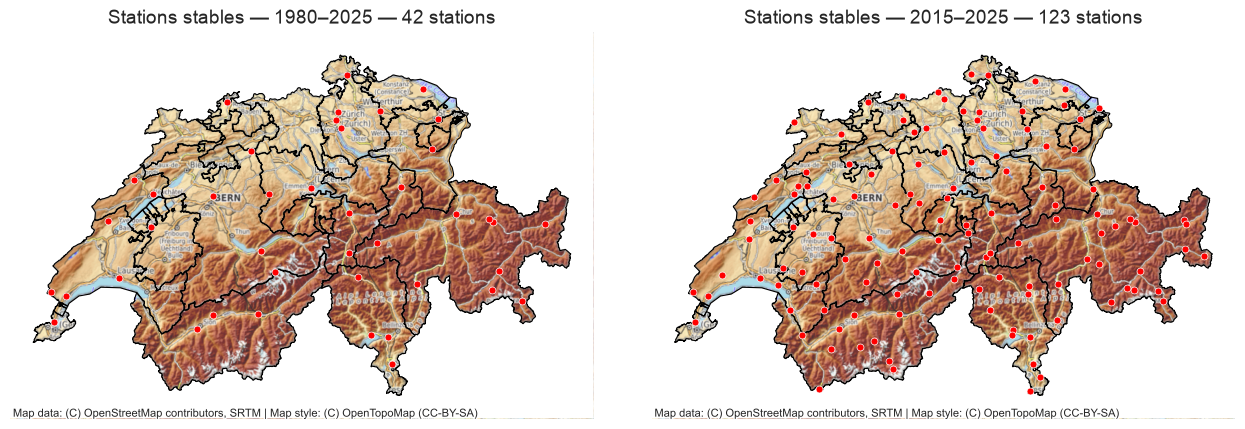
\includegraphics[width=\linewidth,trim=0 0 0 21.6bp,clip]
    {monthly_updated/stations_relief_both_periods.png}
  \caption{Station locations over the Swiss terrain: 1980--2025 (left) and
  2015--2025 (right).}
  %The elevation classes used in the profiles are
  %below 400~m, 400--$<$800~m, 800--$<$1200~m and at least 1200~m.
  \label{fig:stations-relief}
\end{figure}

\clearpage
\subsection{North--south comparison}
\label{subsec:monthly-historical-north-south}
\label{subsec:monthly-recent-north-south}

\savedfigure{monthly_updated/1980_2025_monthly_north_south.png}
{Monthly profiles by latitude group, 1980--2025.}
{fig:monthly-historical-north-south}

\savedfigure{monthly_updated/2015_2025_monthly_north_south.png}
{Monthly profiles by latitude group, 2015--2025.}
{fig:monthly-recent-north-south}

\savedfigure{monthly_updated/stations_north_south_both_periods.png}
{North--south stratification for 1980--2025 (left) and 2015--2025 (right).}
% The blue dashed line follows latitude $46.8^\circ$N.
% Stations with latitude strictly above $46.8^\circ$N belong to the North
% group; all other stations belong to the South group.
{fig:stations-north-south}

\clearpage
\begingroup
\setlength{\intextsep}{6pt}
\subsection{Four geographic sectors}
\label{subsec:monthly-historical-geographic}
\label{subsec:monthly-recent-geographic}

\savedfigure{monthly_updated/1980_2025_monthly_geographic.png}
{Monthly profiles by geographic sector, 1980--2025.}
{fig:monthly-historical-geographic}

\savedfigure{monthly_updated/2015_2025_monthly_geographic.png}
{Monthly profiles by geographic sector, 2015--2025.}
{fig:monthly-recent-geographic}

\savedfigure{monthly_updated/stations_geographic_both_periods.png}
{Four-sector stratification for 1980--2025 (left) and 2015--2025 (right).}
% The common centre is the mean latitude and longitude of all reference
% stations in the full dataset. With $x=(\lambda-\lambda_0)\cos\varphi_0$
% and $y=\varphi-\varphi_0$, the dashed boundaries follow $y=\pm x$.
% When $|y|\geq|x|$, stations are assigned to North or South according
% to the sign of $y$ (zero belongs to North); otherwise they are assigned
% to East or West according to the sign of $x$.
{fig:stations-geographic}

\endgroup

\appendix
\clearpage
\section{Station coverage}
\subsection{Network development}
The bar charts below show an increase from 72 wind stations in 1980 to
about 150 in 2025, and from 50 solar stations in 1981 to about 134 in 2025.
Wind coverage rises sharply around 1993, while solar coverage expands strongly after 2008.

\savedfigure{station_coverage_wind.png}
{Stations with at least one daily wind measurement in each year.}
{fig:coverage-wind}
\savedfigure{station_coverage_solar.png}
{Stations with at least one daily solar-radiation measurement in each year.}
{fig:coverage-solar}

\end{document}
